\subsection{The Life Cycle of an SGX Enclave}
\label{sec:sgx_enclave_lifecycle}

An enclave's life cycle is deeply intertwined with resource management,
specifically the allocation of EPC pages. Therefore, the instructions that
transition between different life cycle states can only be executed by the
system software. The system software is expected to expose the SGX instructions
described below as enclave loading and teardown services.

The following subsections describe the major steps in an enclave's lifecycle,
which is illustrated by Figure~\ref{fig:sgx_enclave_lifecycle}.

\begin{figure}[hbt]
  \centering
  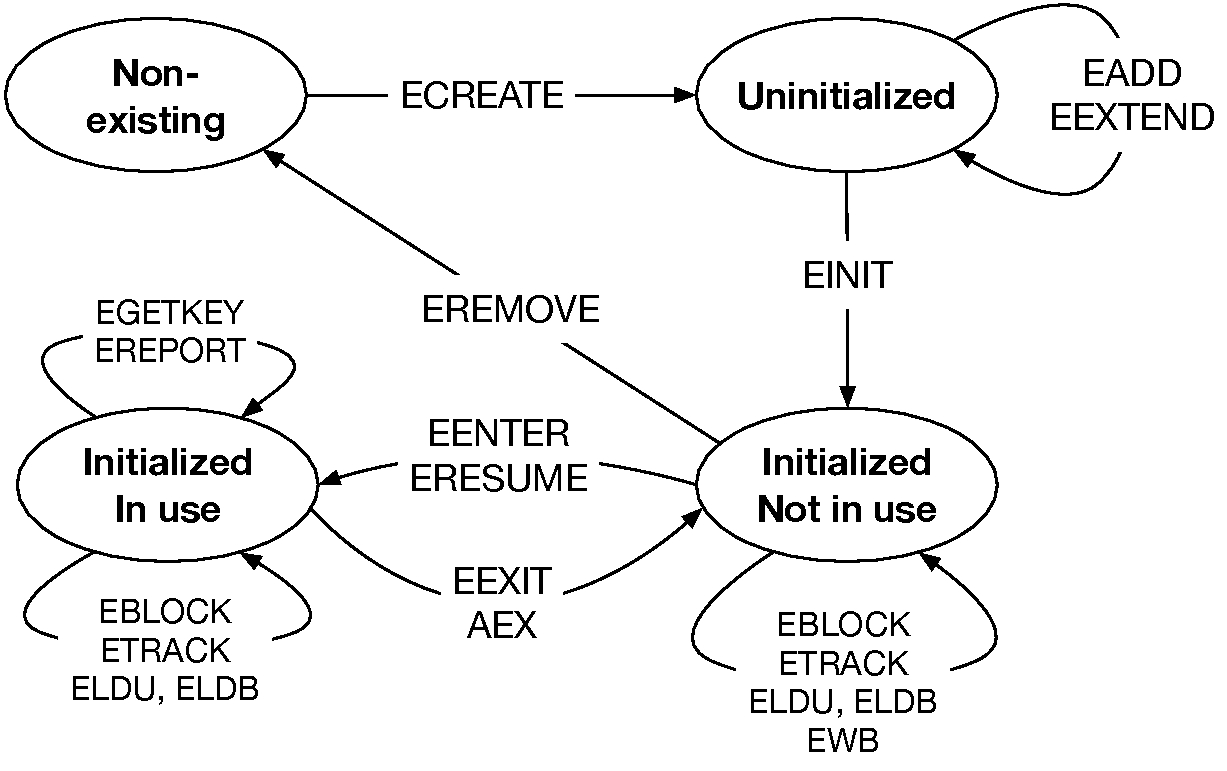
\includegraphics[width=85mm]{figures/sgx_enclave_lifecycle.pdf}
  \caption{
    The SGX enclave life cycle management instructions and state transition
    diagram
  }
  \label{fig:sgx_enclave_lifecycle}
\end{figure}


% Enclave Entry and Exiting : SDM S 39.2, S 39.2.1
% ECREATE, EADD, EREMOVE: SDM S 41.3

\subsubsection{Creation}
\label{sec:sgx_ecreate}

An enclave is born when the system software issues the \texttt{ECREATE}
instruction, which turns a free EPC page into the SECS~(\S~\ref{sec:sgx_secs})
for the new enclave.

\texttt{ECREATE} initializes the newly created SECS using the information in a
non-EPC page owned by the system software. This page specifies the values for
all the SECS fields defined in the SDM, such as BASEADDR and SIZE, using an
architectural layout that is guaranteed to be preserved by future
implementations.

While is very likely that the actual SECS layout used by initial SGX
implementations matches the architectural layout quite closely, future
implementations are free to deviate from this layout, as long as they maintain
the ability to initialize the SECS using the architectural layout.
Software cannot access an EPC page that holds a SECS, so it cannot become
dependent on an internal SECS layout. This is a stronger version of the
encapsulation used in the Virtual Machine Constrol
Structure~(VMCS,~\S~\ref{sec:vmx}).

\texttt{ECREATE} validates the information used to initialize the SECS, and
results in a page fault~(\#PF,~\S~\ref{sec:faults}) or general protection
fault~(\#GP,~\S~\ref{sec:faults}) if the information is not valid. For example,
if the SIZE field is not a power of two, \texttt{ECREATE} results in \#GP. This
validation, combined with the fact that the SECS is not accessible by software,
simplifies the implementation of the other SGX instructions, which can assume
that the information inside the SECS is valid.


\subsubsection{Loading}
\label{sec:sgx_eadd}

\texttt{ECREATE} marks the newly created SECS as \textit{uninitialized}. While
an enclave's SECS is in this state, the system software can use \texttt{EADD}
instructions to load the initial code and data into the enclave. \texttt{EADD}
is used to create both TCS pages (\S~\ref{sec:sgx_tcs}) and regular pages.

% Page Information (PAGEINFO): SDM S 38.10
% Security Information (SECINFO): SDM S 38.11

\texttt{EADD} reads its input data from a \textit{Page Information}~(PAGEINFO)
structure, illustrated in Figure~\ref{fig:sgx_pageinfo}. The structure's
contents is only used to communicate information to the SGX implementation, so
it is entirely architectural and documented in the SDM.

\begin{figure}[hbt]
  \centering
  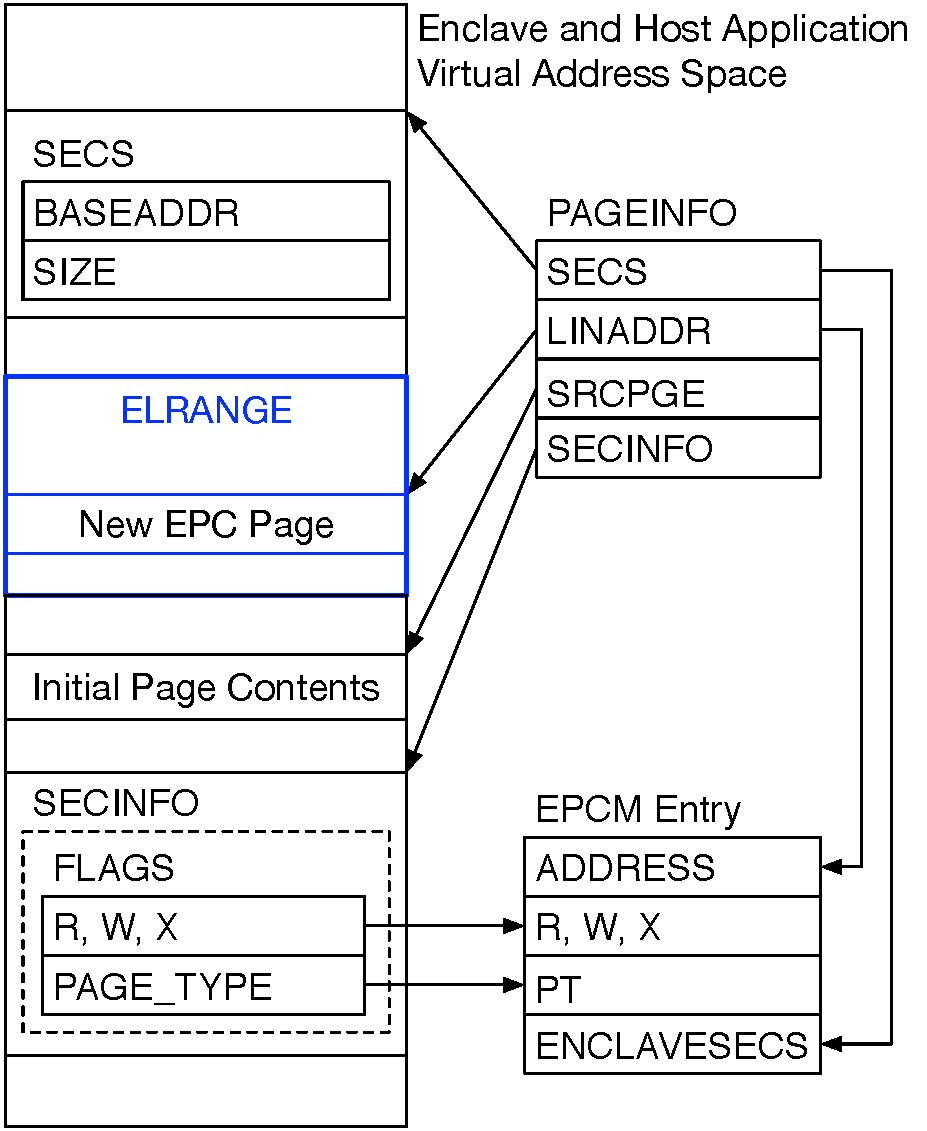
\includegraphics[width=65mm]{figures/sgx_pageinfo.pdf}
  \caption{
    The PAGEINFO structure supplies input data to SGX instructions such as
    \texttt{EADD}.
  }
  \label{fig:sgx_pageinfo}
\end{figure}

Currently, the PAGEINFO structure contains the virtual address of the EPC page
that will be allocated (LINADDR), the virtual address of the non-EPC page whose
contents will be copied into the newly allocated EPC page (SRCPGE), a virtual
address that resolves to the SECS of the enclave which will own the page
(SECS), and values for some of the fields of the EPCM entry associated with the
newly allocated EPC page (SECINFO).

The SECINFO field in the PAGEINFO structure is actually a virtual memory
address, and points to a \textit{Security Information}~(SECINFO) structure,
some of which is also illustrated in Figure~\ref{fig:sgx_pageinfo}. The SECINFO
structure contains the newly allocated EPC page's access permissions (R, W, X)
and its EPCM page type (PT\_REG or PT\_TCS). Like PAGEINFO, the SECINFO
structure is solely used to communicate data to the SGX implementation, so it
its contents is also entirely architectural. However, most of the structure's
64 bytes are reserved for future use.

Both the PAGEINFO and the SECINFO structures are prepared by the system
software that invokes the \texttt{EADD} instruction, and therefore must be
contained in non-EPC pages. Both structures must be aligned to their sizes --
PAGEINFO is 32 bytes long, so each PAGEINFO instance must be 32-byte aligned,
while SECINFO has 64 bytes, and therefore each SECINFO instance must be
64-byte aligned. The alignment requirements likely simplify the SGX
implementation by reducing the number of special cases that must be handled.

\texttt{EADD} validates its inputs before modifying the newly allocated EPC
page or its EPCM entry. Most importantly, attempting to \texttt{EADD} a page to
an enclave whose SECS is in the initialized state will result in \#GP.
Furthermore, attempting to \texttt{EADD} an EPC page that is already allocated
(the VALID field in its EPCM entry is 1) results in \#PF. \texttt{EADD} also
ensures that the page's virtual address falls within the enclave's ELRANGE, and
that all the reserved fields in SECINFO are set to zero.

While loading an enclave, the system software will also use the
\texttt{EEXTEND} instruction, which updates the enclave's measurement used in
the software attestation process. Software attestation is discussed in
\S~\ref{sec:sgx_attestation}.


\subsubsection{Initialization}
\label{sec:sgx_einit_overview}

% EINIT Token Structure (EINITTOKEN): SDM S 38.14

After loading the initial code and data pages into the enclave, the system
software must use a \textit{Launch Enclave}~(LE) to obtain an EINIT Token
Structure, via an under-documented process that will be described in more
detail in \S~\ref{sec:sgx_einit}. The token is then provided to the
\texttt{EINIT} instruction, which marks the enclave's SECS as
\textit{initialized}.

The LE is a privileged enclave provided by Intel, and \textbf{is a prerequisite
for the use of enclaves authored by parties other than Intel}. The LE is an
SGX enclave, so it must be created, loaded and initialized using the processes
described in this section. However, the LE is cryptographically
signed~(\S~\ref{sec:integrity_crypto}) with a special Intel key that is
hard-coded into the SGX implementation, and that causes \texttt{EINIT} to
initialize the LE  without checking for a valid EINIT Token Structure.

After \texttt{EINIT} is successfully called on an enclave,
ring 3~\S~\ref{sec:rings}) application software can execute the enclave's code,
using the SGX instructions described in \S~\ref{sec:sgx_threads}. On the other
hand, once an enclave's SECS is marked as \textit{initialized}, \texttt{EADD}
cannot be invoked on that enclave anymore, so the system software must load all
the pages that make up the enclave's initial state before executing the
\texttt{EINIT} instruction.


\subsubsection{Teardown}
\label{sec:sgx_eremove}

After the enclave has done the computation it was designed to perform, the
system software executes the \texttt{EREMOVE} instruction to deallocate the
EPC pages used by the enclave.

\texttt{EREMOVE} marks an EPC page as available by setting the VALID field of
the page's EPCM entry to 0 (zero). Before freeing up the page, \texttt{EREMOVE}
makes sure that there is no logical processor executing code inside the enclave
that owns the page to be removed.

An enclave is completely destroyed when the EPC page holding its SECS is freed.
\texttt{EREMOVE} refuses to deallocate a SECS page if it is referenced by any
other EPCM entry's ENCLAVESECS field, so an enclave's SECS page can only be
deallocated after all the enclave's pages have been deallocated.
